
\section{Interface Graphique}
\par L'interface graphique de notre application se décompose en 3 composants principaux :
\begin{itemize}
    \item Le Menu
    \item La fenêtre principale de l'application
    \item La fenêtre de chargement d'un modèle
\end{itemize}
\subsection{Menu}
\par Le Menu est la page d'accueil de l'application, il sert à choisir le type d'automate cellulaire souhaité pour la simulation de notre "Game of life". Le choix de l'automate cellulaire ce fait grâce aux boutons :
\begin{itemize}
    \item \textbf{Hashlife} bouton (initialise un automate cellulaire utilisant l'algorithme hahslife)
    \item \textbf{Margolus} bouton (initialise un automate cellulaire utilisant les algorithmes de margolus)
    \item \textbf{Neural} bouton (initialise un automate cellulaire utilisant les algorithmes neuronaux)
\end{itemize}

\begin{figure}[H]
    \centering
    
\includegraphics[width=0.5\textwidth]{images/imgInterface/boutons.png}
    \caption{Bouton Hashlife du menu}
    \label{fig:hashlife bouton}
\end{figure}

\par Chaque bouton est accompagné sur sa droite d'un bouton d'information. Chaque bouton ouvre une fenêtre pop-up contenant un lien qui renvoie vers un site permettant d'avoir plus d'informations sur l'option à sa gauche.

\begin{figure}[H]
    \centering
    
\includegraphics[width=0.5\textwidth]{images/imgInterface/boutonInformation.png}
    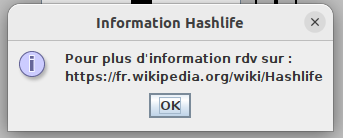
\includegraphics[width=0.5\textwidth]{images/imgInterface/popup.png}
    \caption{Bouton d'information de Hashlife}
    \label{fig:bouton info}
\end{figure}

\subsection{Fenêtre principale}
\par La fenêtre principale permet l'affichage de l'automate cellulaire ainsi que son contrôle grâce de multiples boutons présent sur une \textbf{JToolBar} : la barre d'options

\subsubsection{Barre d'option}

\par La barre d'option contient 10 boutons :
\begin{itemize}
    \item \textbf{Home} (permet de revenir dans le menu pour changer d'automate cellulaire)
    
    \item \textbf{Move} (permet de ce déplacer dans l'affichage de l'automate et de zoomer)
    
    \item \textbf{Secret} (je vous laisse découvrir le secret par vous même)
    
    \item \textbf{Rule} (affiche la règle courante suivit par l'automate cellulaire)
    
    \item \textbf{Choix rules} (un menu déroulant contenant les différentes règles que l'automate peut suivre (change en fonction de l'automate))
    
    \item \textbf{Play} (permet de lancer/mettre en pause la simulation de l'automate cellulaire)
    
    \item \textbf{Random} (permet de remplir l'automate cellulaire aléatoirement)
    
    \item \textbf{Clear} (permet de vider l'automate cellulaire)
    
    \item \textbf{Speed} (permet d'accélérer la vitesse de la simulation, il n'est disponible que si l'automate utilise l'algorithme hashlife)
    
    \item \textbf{Modele} (un menu déroulant contenant différents modèle importable du jeu de la vie (les modèles changent en fonction de l'automate initialisé)
\end{itemize}

\begin{figure}[H]
    \centering
    
\includegraphics[width=1\textwidth]{images/imgInterface/optionBar.png}
    \caption{Barre d'options}
    \label{fig:barre d'options} 
\end{figure}

\subsubsection{Affichage automate}
\par Comme dis précédemment l'affichage automate affiche la simulation du jeu de la vie en cours. Dans cette affichage vous pouvez cliquer affin d'ajouter une cellule vivante (représenter par un pixel noir) sur l'endroit cliqué. Pour se déplacer et zoomer dans l'affichage c'est très simple :

\begin{itemize}
    \subsubsection{Déplacement}
    \item \textbf{z/Z} déplacement vers l'avant
    \item \textbf{q/Q} déplacement vers la gauche
    \item \textbf{d/D} déplacement vers la droite
    \item \textbf{s/S} déplacement vers l'arrière
    \subsubsection{Zoom}
    \item \textbf{a/A} zoom +
    \item \textbf{e/E} zoom -
\end{itemize}{}

\begin{figure}[H]
    \centering
    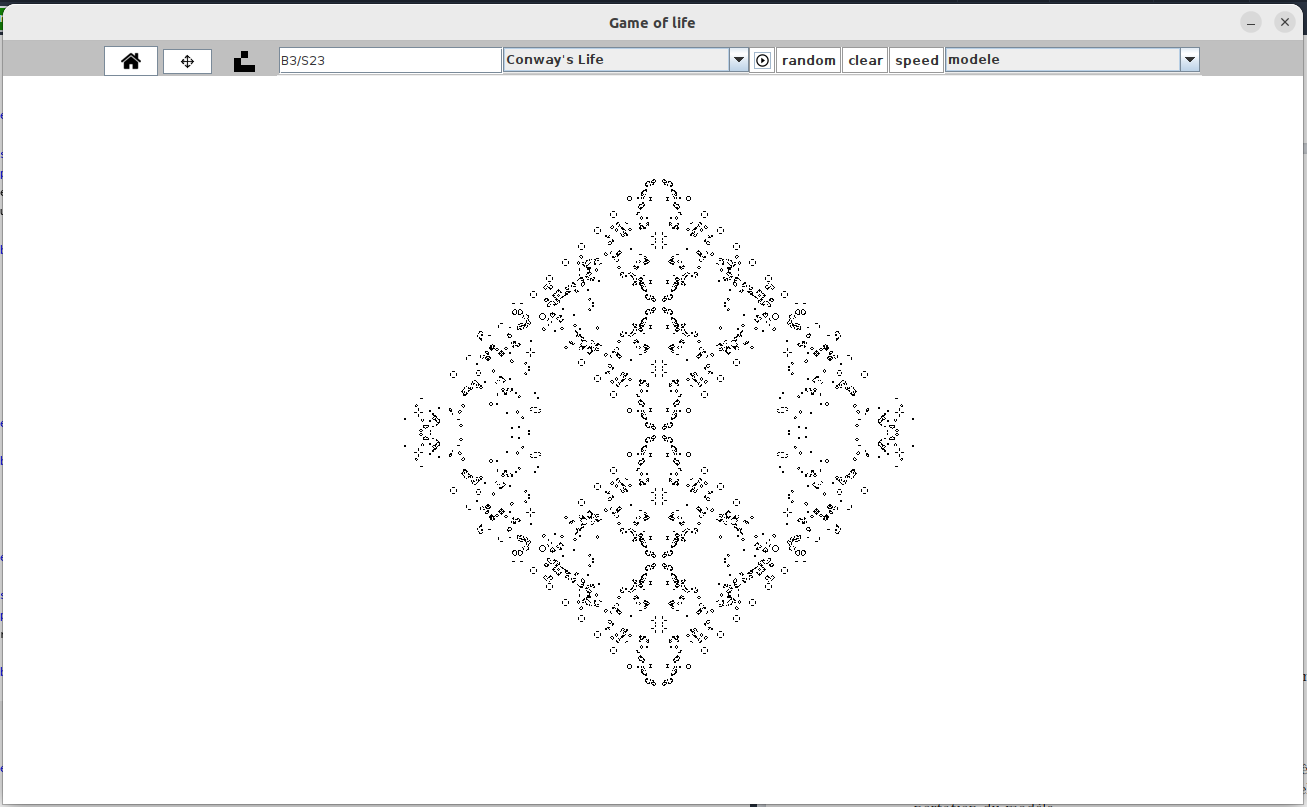
\includegraphics[width=0.5\textwidth]{images/imgInterface/simulation2.png}
    \caption{Affichage d'une simulation}
    \label{fig:simulation} 
\end{figure}

\subsection{Fenêtre de chargement}
\par Lorsque l'on importe un nouveau modèle alors la fenêtre de chargement s'ouvre et une barre de progression est affiché. La barre selon le niveau d'importation du modèle.

\begin{figure}[H]
    \centering
    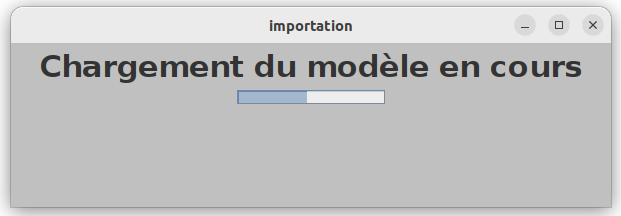
\includegraphics[width=0.5\textwidth]{images/imgInterface/chargement.png}
    \caption{Fenêtre de chargement}
    \label{fig:chargement} 
\end{figure}
